\documentclass{beamer}
%
% Choose how your presentation looks.
%
% For more themes, color themes and font themes, see:
% http://deic.uab.es/~iblanes/beamer_gallery/index_by_theme.html
%

\mode<presentation>
{
  \usetheme{Darmstadt}      % or try Darmstadt, Madrid, Warsaw, ...
  \usecolortheme{beaver} % or try albatross, beaver, crane, ...
  \usefonttheme{default}  % or try serif, structurebold, ...
  \setbeamertemplate{navigation symbols}{}
  \setbeamertemplate{caption}[numbered]
} 

\usepackage[backend=bibtex]{biblatex}
\addbibresource{bibliography.bib}

\usepackage[english]{babel}
\usepackage[utf8x]{inputenc}
\usebackgroundtemplate{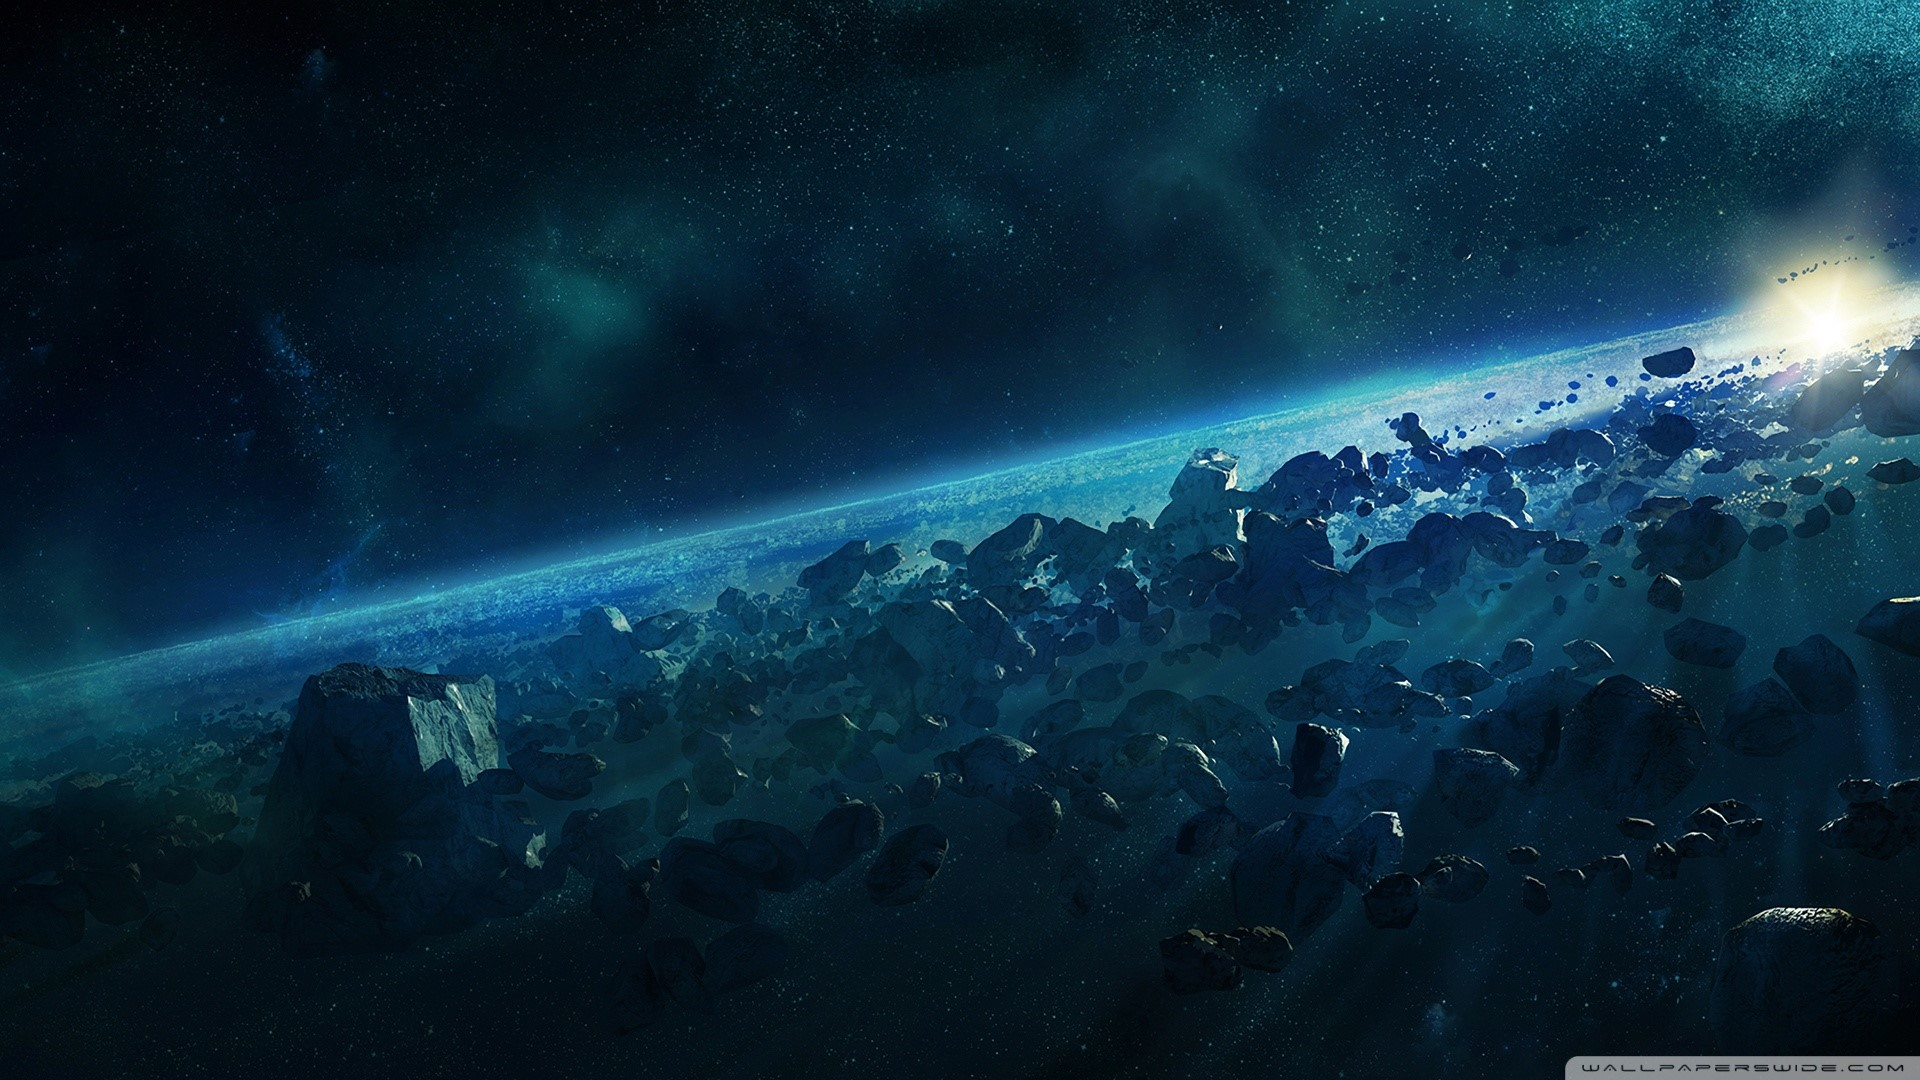
\includegraphics[width=\paperwidth]{Pic/Intro.jpg}}
\title[Hazardous asteroids forecast via Markov random fields]{Hazardous asteroids forecast via Markov random fields}
\subtitle{Project for the exam: Probabilistic Modelling (DSE)}
\author{Marzio De Corato}
\date{\today}

\begin{document}

\begin{frame}
\vspace{+4 cm}  \titlepage
\end{frame}

\usebackgroundtemplate{ } 

% Uncomment these lines for an automatically generated outline.
%\begin{frame}{Outline}
%  \tableofcontents
%\end{frame}

\section{Intro}

\begin{frame}{Introduction}

\begin{itemize}
\item \textbf{Final Goal} Assessment of forecasts and interpretability for different machine learning algorithms, including the probabilistic models
\item \textbf{Method} Use a dataset for which the laws that interconnects the different features are known from general principles
\item \textbf{Dataset} CNEOS asteroids dataset for more than 3500 asteroids
\item \textbf{Theoretical laws} Celestial mechanics
\item \textbf{Algorithms involved - probabilistic models} GLASSO, mgm, minforest, mmod
\item \textbf{Algorithms involved - others} Random forest, Support Vector Machines, Quadratic Discriminant Analysis, Logistic Regression  

\end{itemize} 

\end{frame}

\section{Celestial mechanics}

\begin{frame}{Celestial mechanics}
\begin{equation}
\textbf{F}_{1}=\mathcal{G} \cdot \frac{m_{1}m_{2}}{r^{3}}\textbf{r}=m_{1} \ddot{\textbf{r}}_{1}
\end{equation}

\begin{equation}
\textbf{F}_{2}=-\mathcal{G} \cdot \frac{m_{1}m_{2}}{r^{3}}\textbf{r}=m_{1} \ddot{\textbf{r}}_{2}
\end{equation}
 
If we consider the motion of the second item with respect to the first one 
 
\begin{equation}
\ddot{\textbf{r}}=\ddot{\textbf{r}}_{2}-\ddot{\textbf{r}}_{1} \quad \mu=\mathcal{G}(m_{1}+m_{2})
\end{equation}

\begin{equation}
\dfrac{d^{2}\textbf{r}}{dt^{2}}+\mu\dfrac{\textbf{r}}{r^{3}}=0
\end{equation}

$\textbf{r} \times \ddot{ \textbf{r}}=0  \implies $ $\textbf{r}$  and $\dot{\textbf{r}}$ lies in the same plane

\end{frame}

\begin{frame}{Celestial mechanics}
With polar coordinates  $\hat{\textbf{r}}$ and $\hat{\boldsymbol{\theta}}$

\begin{equation}
\textbf{r}=r\hat{\textbf{r}}
\end{equation}

\begin{equation}
\dot{\textbf{r}}=\dot{r}\hat{\textbf{r}}+r\dot{\theta}\hat{\boldsymbol{\theta}}
\label{eq_dyn_nop}
\end{equation}

\begin{equation}
\ddot{\textbf{r}}=\left(\ddot{r}-r\dot{\theta}^{2}\right)\hat{\textbf{r}}+\left[\dfrac{1}{r}\frac{d}{dt}\left(r^{2}\dot{\theta}\right)\right]\hat{\boldsymbol{\theta}}
\end{equation}

\begin{equation}
\textbf{h}=r^{2}\dot{\theta}\hat{\textbf{z}}
\end{equation}


\begin{equation}
h=r^{2}\dot{\theta}
\end{equation}

\end{frame}


\begin{frame}{Celestial mechanics \cite{murray1999solar}: $2^{th}$ Kepler law}

\begin{figure}[h]
\begin{center}
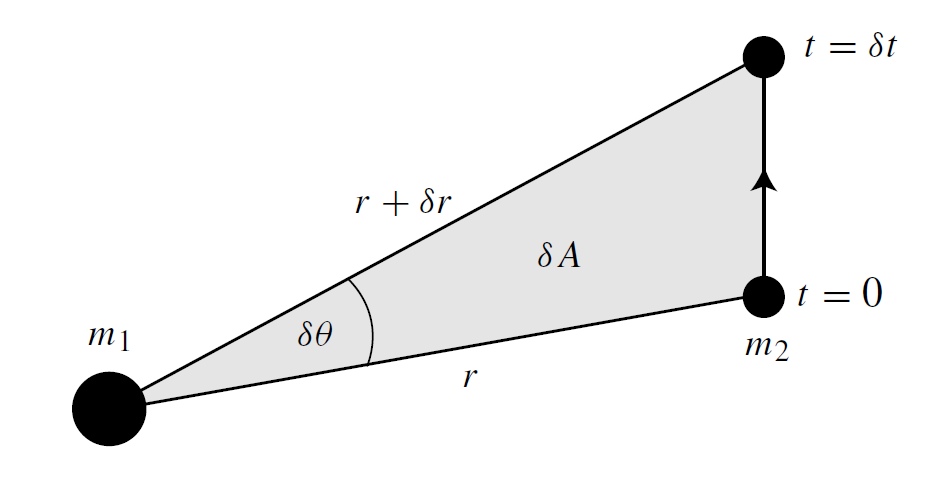
\includegraphics[width=0.3\textwidth]{Pic/Area_dynamics.png}
\caption{\cite{murray1999solar}}
\label{Area_dynamics}
\end{center}
\end{figure}

\begin{equation}
\delta A \approx \dfrac{1}{2} r(r+dr)\sin(\delta\theta) \approx  \dfrac{1}{2} r^{2}\delta\theta
\end{equation}

\begin{equation}
\dfrac{dA}{dt}=\dfrac{1}{2}r^{2}\dfrac{d\theta}{dt}=\dfrac{1}{2}h
\end{equation}

\begin{center}
$h$ is constant $\implies$ $2^{th}$ Kepler law
\end{center}


\end{frame}



\begin{frame}{Celestial mechanics \cite{murray1999solar}: $1^{th}$ Kepler law}
\begin{center}
Using the substitution $u=\dfrac{1}{r}$ $h=r^{2}\dot{\theta}$
\end{center}

\begin{equation}
\dot{r}=-\frac{1}{u}\dfrac{du}{d\theta}\dot{\theta}=-h\frac{du}{d\theta}
\end{equation}

\begin{equation}
\ddot{r}=-h\dfrac{d^{2}u}{d\theta^{2}}\dot{\theta}=-h^{2}u^{2}\frac{d^{2}u}{d\theta^{2}}
\end{equation}

\begin{equation}
\dfrac{d^{2}u}{d\theta^{2}}+u=\frac{\mu}{h^{2}}
\end{equation}

\begin{equation}
u=\frac{\mu}{h^{2}}\left[1+e\cos(\theta-\phi)\right]
\end{equation}

\end{frame}


\begin{frame}{Celestial mechanics \cite{murray1999solar}: $1^{th}$ Kepler law}
\begin{columns}
\column{0.5\textwidth}
\begin{equation}
r=\dfrac{p}{1+e\cos(\theta-\phi)}
\end{equation}


\begin{center}
$e$ is \textcolor{red}{eccentricity}
\end{center}

\begin{itemize}
\item circle:  $e=0$ \quad $p=a$
\item ellipse: $0<e<1$ \quad $p=a(1-e^{2})$
\item parabola: $e=1$ \quad $p=2q$
\item hyperbola: $e>1$ \quad $p=a(e^{2}-1)$
\end{itemize}
\begin{center}
$a$ is the  \textcolor{red}{semi-major axis} of the conic
\end{center}
\column{0.4\textwidth}
\begin{figure}[h]
\begin{center}
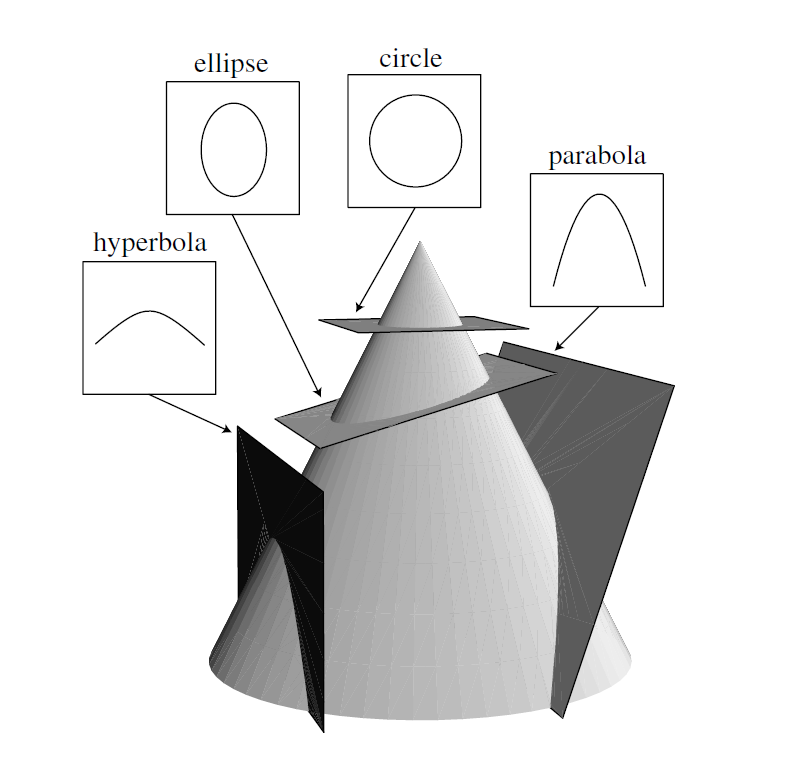
\includegraphics[width=\textwidth]{Pic/Conics.png}
\caption{\cite{murray1999solar}}
\label{Area_dynamics}
\end{center}
\end{figure}

\end{columns}
\end{frame}

\begin{frame}{Celestial mechanics \cite{murray1999solar}: $3^{th}$ Kepler law}
\begin{columns}
\column{0.4\textwidth}

\begin{figure}[h]
\begin{center}
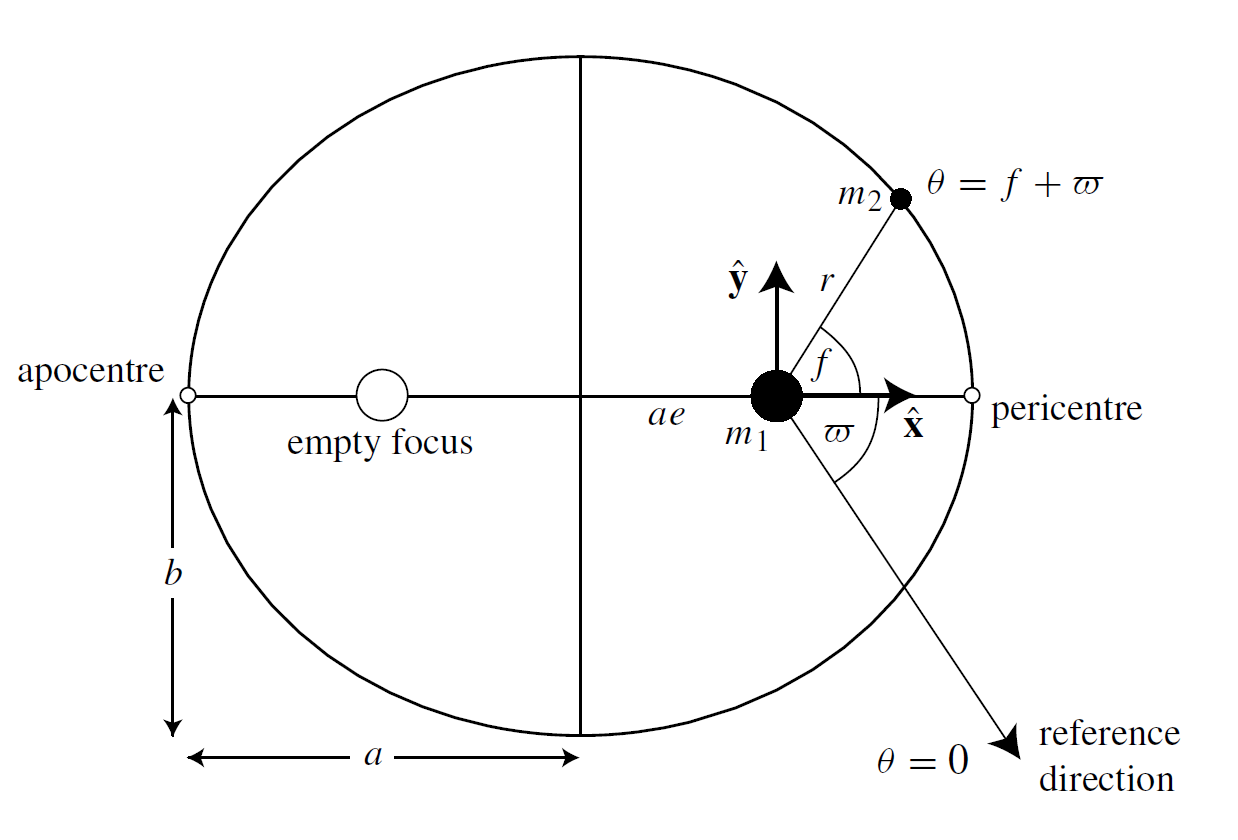
\includegraphics[width=\textwidth ]{Pic/Elliptical_orbit.png}
\caption{\cite{murray1999solar}}
\label{Area_dynamics}
\end{center}
\end{figure}


\column{0.6\textwidth}
\begin{equation}
b^{2}=a^{2}(1-e^{2})
\end{equation}


\begin{equation}
r=\frac{a(1-e^{2})}{1+e\cdot cos(\theta-\phi)}
\label{eq-mot}
\end{equation}

\begin{center}
Area swept in one \textcolor{red}{orbital period} T 
\end{center} 
\begin{center}
$A=\pi ab$
\end{center} 
\begin{center}
We know that: $hT/2 \quad h^{2}=\mu a(1-e^{2})$ 
\end{center}
\begin{center}
Therefore 
\end{center}
\begin{equation}
T^{2}=\dfrac{4\pi^{2}}{\mu}a^{3}
\end{equation}

\end{columns}
\end{frame}

\begin{frame}{$3^{th}$ Kepler law}


\begin{equation}
\frac{m_{c}+m}{m_{c}+m'}=\left(\frac{a}{a'}\right)\left(\frac{T'}{T}\right)^{2}
\end{equation}

But since $m$,$m'<<m_{c}$

\begin{equation}
(a\a')^{3}\approx (T\T')^{2}
\end{equation}

And therefore 

\begin{equation}
T'\approx a'^{3/2}
\end{equation}

\begin{center}
The mass of the asteroid is not involve
\end{center}d


\end{frame}

\begin{frame}{Orbital parameters}
\begin{center}
\textcolor{red}{Mean motion}
\end{center}
\begin{equation}
n=\frac{2\pi}{T}
\end{equation}

\begin{equation}
v_{perihelion}=na\sqrt{\dfrac{1+e}{1-e}}
\end{equation}

\begin{equation}
v_{aphelion}=na\sqrt{\dfrac{1-e}{1+e}}
\end{equation}





\end{frame}



\begin{frame}{Orbital parameters}
\begin{columns}
\column{0.4\textwidth}
\begin{figure}[h]
\begin{center}
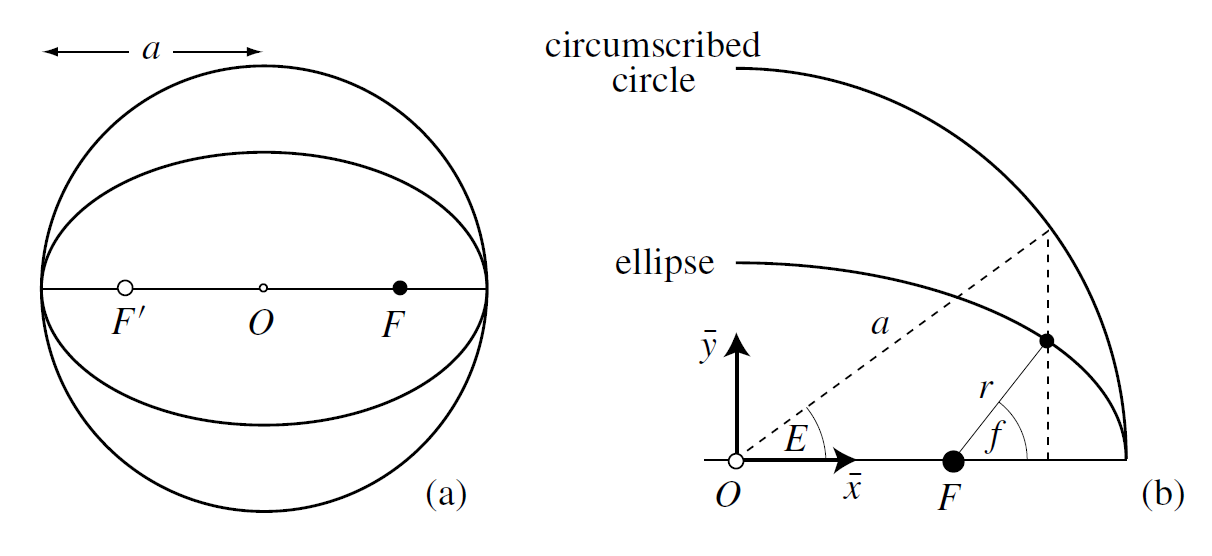
\includegraphics[width=\textwidth ]{Pic/Mean_anomaly.png}
\caption{\cite{murray1999solar}}
\label{Area_dynamics}
\end{center}
\end{figure}
\column{0.6\textwidth}
\begin{center}
\textcolor{red}{Mean anomaly}
\end{center}
\begin{equation}
M=n(t-\tau)
\end{equation}

\begin{center}
\begin{itemize}
\item $M=f=0$\quad$t=\tau$\quad Perihelion
\item $M=f=\pi$\quad$t=\tau+T/2$ \quad Aphelion
\end{itemize}
\end{center}

\begin{equation}
M=E-e\sin E
\end{equation}
\begin{center}
\textcolor{red}{Jupiter Tisserard invariant }
\end{center}
\begin{equation}
T_{P}=\frac{a_{p}}{a}+2\cos I\sqrt{\dfrac{a}{a_{p}}(1-e^{2})}
\end{equation}
\end{columns}
\end{frame}


\begin{frame}{Orbital parameters}
\begin{columns}
\column{0.4\textwidth}
\begin{figure}[h]
\begin{center}
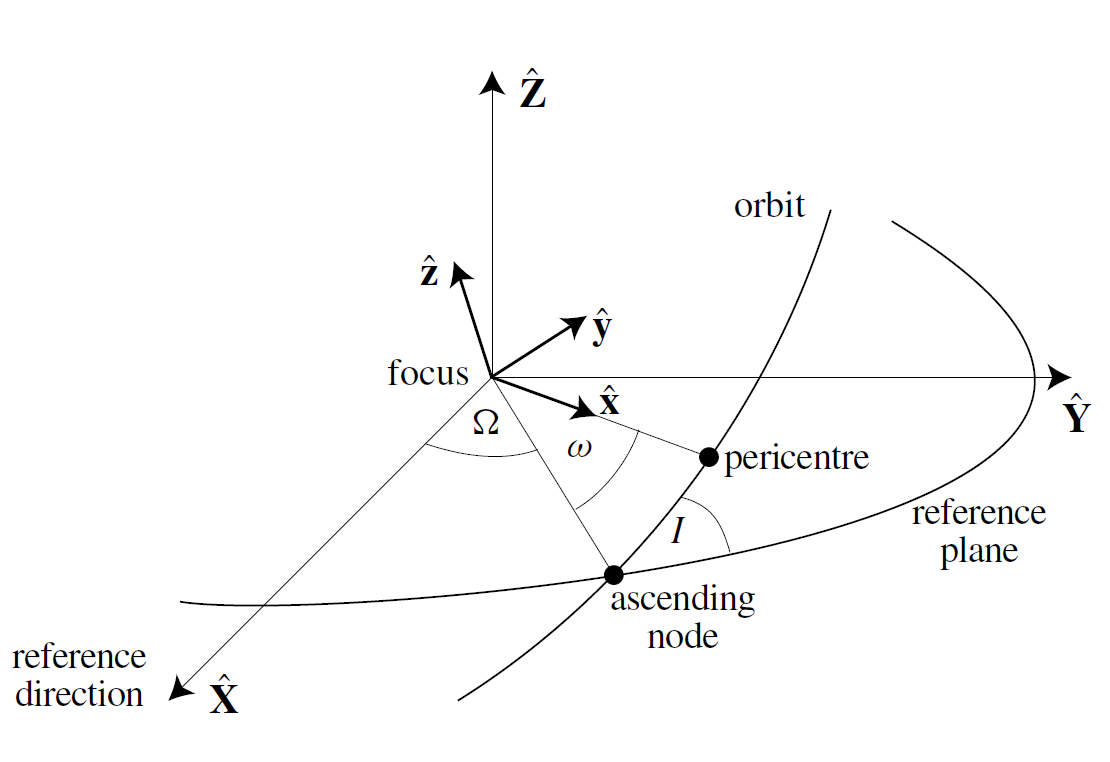
\includegraphics[width=\textwidth ]{Pic/Inclination.png}
\caption{\cite{murray1999solar}}
\label{Area_dynamics}
\end{center}
\end{figure}
\column{0.6\textwidth}
\begin{center}
I: \textcolor{red}{inclination} of the orbit
\end{center}
\begin{center}
$\Omega$: \textcolor{red}{longitude of the ascending node}
\end{center}
\end{columns}
\end{frame}

\begin{frame}{Magnitude}
\begin{equation}
\Phi=\frac{L}{4\pi r^{2}}
\end{equation}
\begin{equation}
m=-2.5\log_{10}\Phi+C
\end{equation}
\begin{equation}
m_{1}-m_{2}=-2.5\log_{10}\frac{\Phi_{1}}{\Phi_{2}}
\end{equation}
\begin{equation}
M-m=-2.5\log_{10}\frac{\Phi\cdot d^{2} }{\Phi\cdot 10^{2}}
\end{equation}
\begin{equation}
M=m+5-5log_{10}d
\end{equation}
Where $\Phi$ is the flux for a sphere of radius r, m the relative magnitude and M the \textcolor{red}{Absolute magnitude}
\end{frame}

\begin{frame}{Magnitude}
\begin{equation}
\Phi=\frac{L}{4\pi r^{2}}
\end{equation}
\begin{equation}
m=-2.5\log_{10}\Phi+C
\end{equation}
\begin{equation}
m_{1}-m_{2}=-2.5\log_{10}\frac{\Phi_{1}}{\Phi_{2}}
\end{equation}
\begin{equation}
M-m=-2.5\log_{10}\frac{\Phi\cdot d^{2} }{\Phi\cdot 10^{2}}
\end{equation}
\begin{equation}
M=m+5-5log_{10}d
\end{equation}
Where $\Phi$ is the flux for a sphere of radius r, m the relative magnitude and M the \textcolor{red}{Absolute magnitude}
\end{frame}

\begin{frame}{Classification}
\begin{figure}[h]
\begin{center}
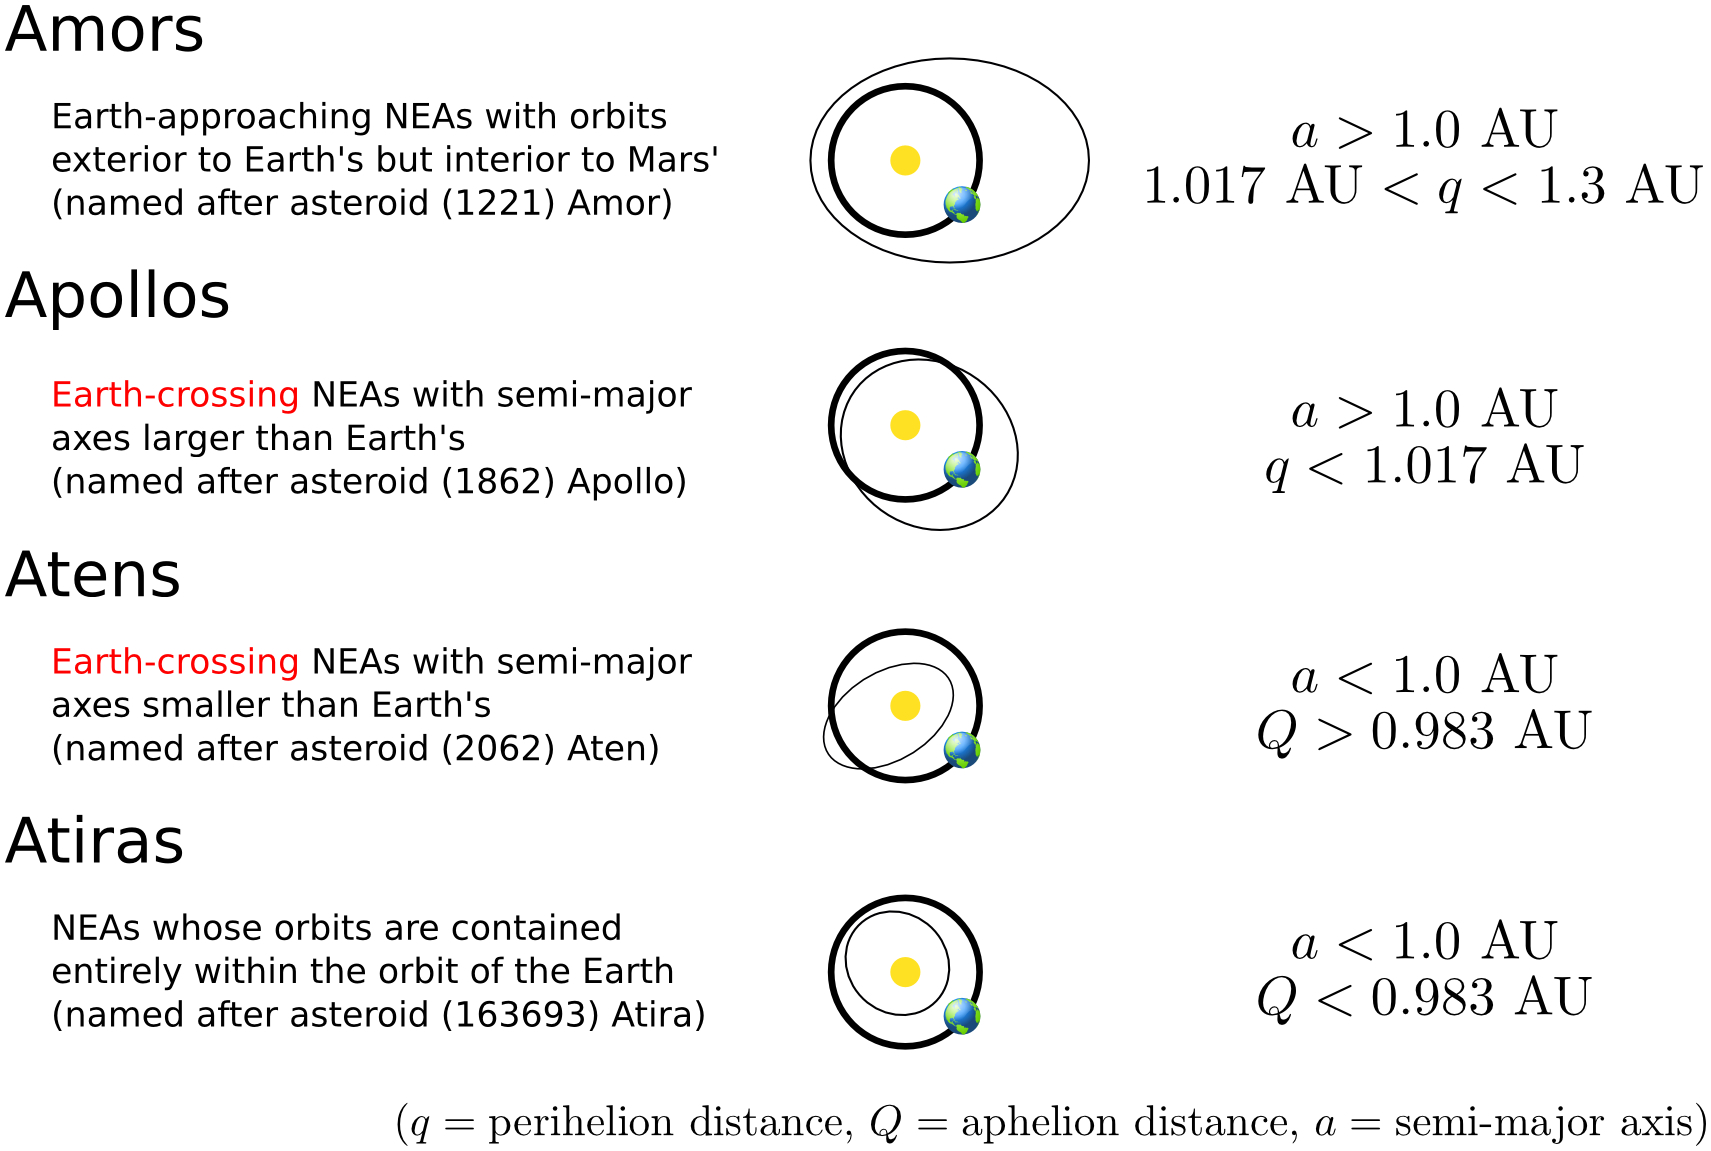
\includegraphics[width=\textwidth]{Pic/neo_orbit_types.jpg}
\caption{\cite{nasa_classification}}
\label{Area_dynamics}
\end{center}
\end{figure}
\end{frame}

\begin{frame}{Classification}
\begin{itemize}
\item \textbf{Potentially Hazardous Asteroids}: MOID $\leq 0.05$ au $M \leq22.0$ \textit{NEAs whose Minimum Orbit Intersection Distance (MOID) with the Earth is 0.05 au or less and whose absolute magnitude (M) is 22.0 or brighter}
\end{itemize}
\end{frame}

\section{Dataset}

\begin{frame}{Classification}
\begin{itemize}


\item The asteroid dataset was retrieved from Kaggle \cite{kaggle_dataset}, which reports into a more machine readable form the dataset of The Center for Near-Earth Object Studies (CNEOS) \cite{cneos+nasa}, a NASA research centre.

\item 3552 Asteroids

\item Among the 40 the features, the ones connected only to the other name of
the asteroid, or connected only to the name of the orbit and
the one connected with the orbiting planet ( since for all it was
the Earth) were discarted

\item The proportion hazardous/not hazardous was set 1:5  

\item The continuous measures were standardised and demeaned

\end{itemize}
\end{frame}

\begin{frame}{Features}
\begin{table}[]
\begin{center}
\begin{tabular}{c|c}
\hline
\textbf{Features}             & \textbf{Type}        \\ \hline
Neo Reference ID              & not used             \\ \hline
Absolute Magnitude            & Continuous           \\ \hline
Est Dia in KM (min)           & Continuous           \\ \hline
Est Dia in KM (max)           & Continuous           \\ \hline
Close Approach Date           & Continuous           \\ \hline
Epoch Date Close Approach     & Continuous           \\ \hline
Relative\_Velocity            & Continuous           \\ \hline
Miss\_Dist                    & Continuous           \\ \hline
Min\_Orbit\_Intersection      & Continuous           \\ \hline
Jupiter\_Tisserand\_Invariant & Continuous           \\ \hline
Epoch\_Osculation             & Continuous           \\ \hline
Eccentricity                  & Continuous           \\ \hline

\end{tabular}
\end{center}
\label{tab_features}
\end{table}

\end{frame}


\begin{frame}{Features}
\begin{table}[]
\begin{center}
\begin{tabular}{c|c}
\hline
\textbf{Features}             & \textbf{Type}        \\ \hline
Semi Major Axis               & Continuous           \\ \hline
Inclination                   & Continuous           \\ \hline
Asc Node Longitude            & Continuous           \\ \hline
Orbital Period                & Continuous           \\ \hline
Perihelion Distance           & Continuous           \\ \hline
Perihelion Arg                & Continuous           \\ \hline
Perihelion Time               & Continuous           \\ \hline
Mean\_Anomaly                 & Continuous           \\ \hline
Mean\_Motion                  & Continuous           \\ \hline
Hazardous                     & Categorical (Binary)
\end{tabular}
\end{center}
\label{tab_features}
\end{table}

\end{frame}


\section{Prelim. analysis}

\begin{frame}
\begin{columns}
\column{0.5\textwidth}
  \begin{figure}[b]{\textwidth}
    \centering
    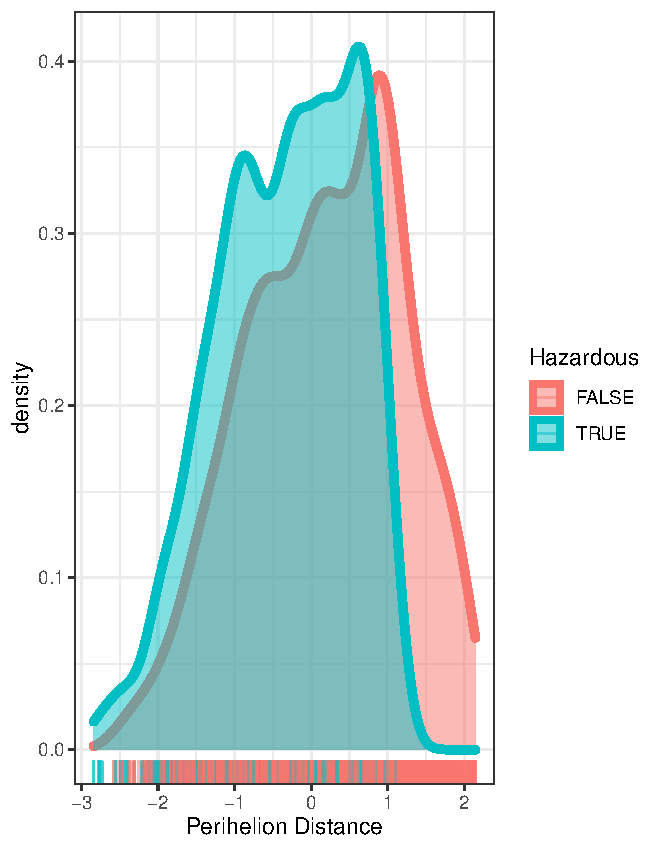
\includegraphics[width=\textwidth]{Pic/DENSITY_Perihelion_Distance.pdf}
    \subcaption{ \begin{center}
    a) Perihelion Distance
    \end{center}}
    \vspace{4ex}
  \end{figure} 
\column{0.5\textwidth}
  \begin{figure}[b]{\textwidth}
    \centering
    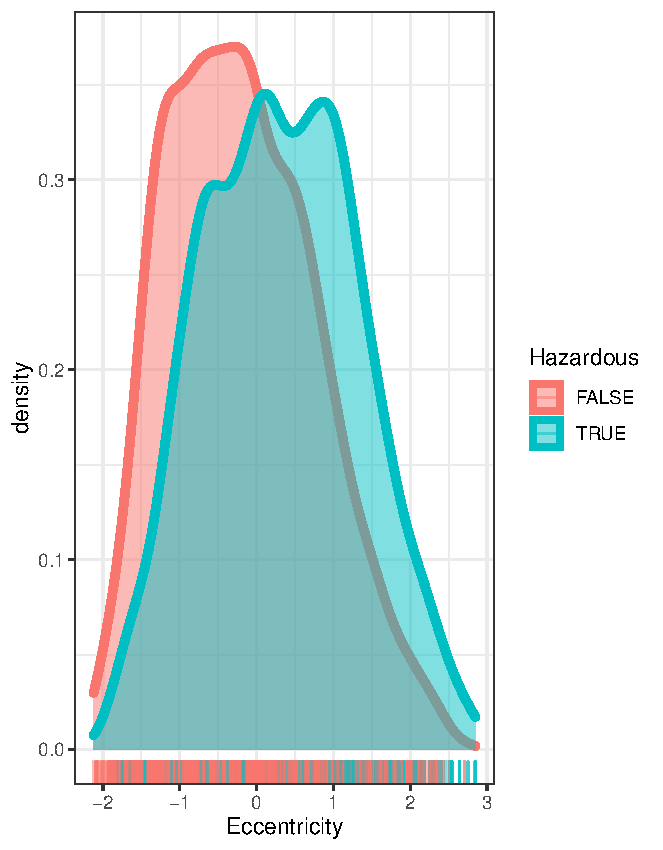
\includegraphics[width=\textwidth]{Pic/DENSITY_Eccentricity.pdf}
    \subcaption{ \begin{center}
    b) Eccentricity
    \end{center}}
    \vspace{4ex}
  \end{figure}
\end{columns}
\end{frame}

\begin{frame}
\begin{columns}  

\column{0.5\textwidth}
    \begin{figure}[b]{\textwidth}
    \centering
    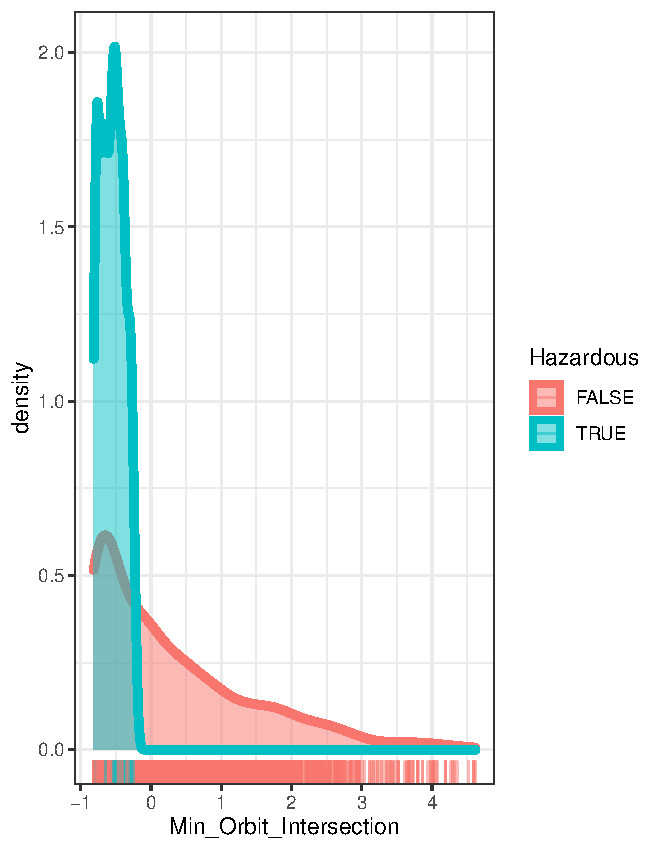
\includegraphics[width=\textwidth]{Pic/DENSITY_Min_orbit_intersection.pdf}
    \subcaption{ \begin{center}
    c) Min orbit intersection
    \end{center}}
    \vspace{4ex}
  \end{figure}
  \column{0.5\textwidth}
  \begin{figure}[b]{\textwidth}
    \centering
    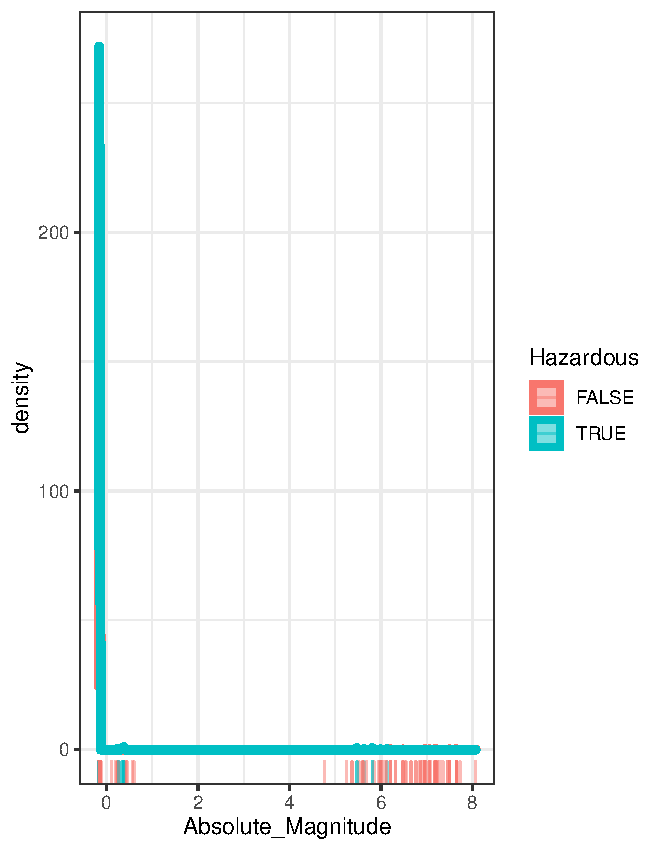
\includegraphics[width=\textwidth]{Pic/DENSITY_Absolute_magnitude.pdf}
    \subcaption{ \begin{center}
    d) Absolute magnitude
    \end{center}}
    \vspace{4ex}
  \end{figure}
\end{columns}
\end{frame}


\begin{frame}{FAMD}
\begin{columns}  

\column{0.5\textwidth}
    \begin{figure}[h]
\begin{center}
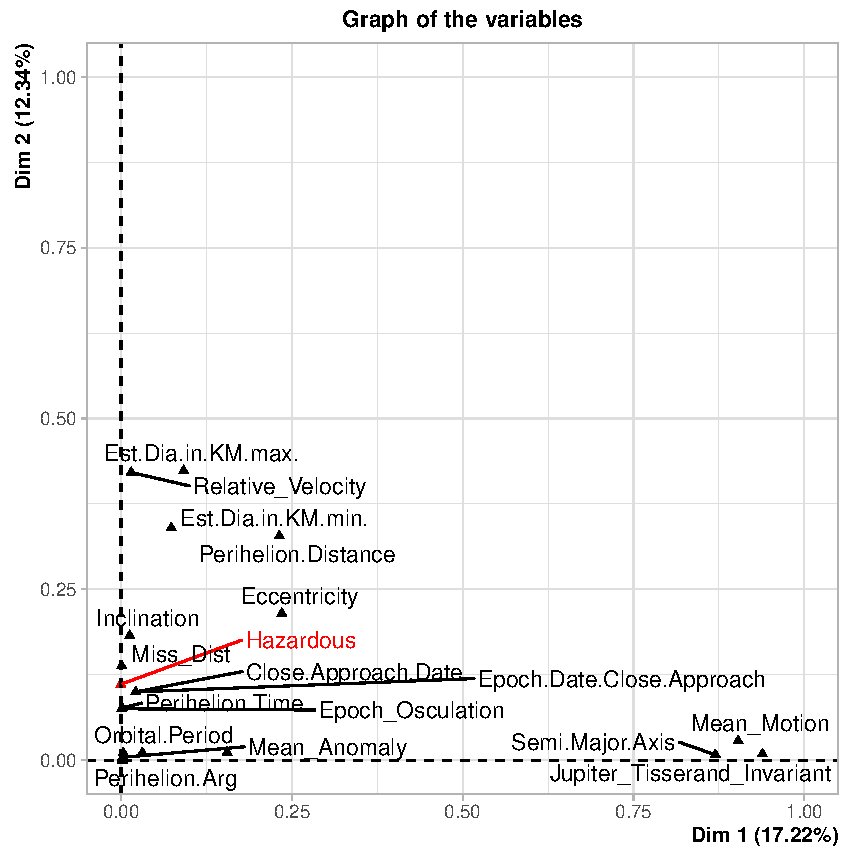
\includegraphics[width=1\textwidth]{Pic/FAMD.pdf}
\label{FADM}
\end{center}
\end{figure}
  \column{0.5\textwidth}
 \begin{figure}[h]
\begin{center}
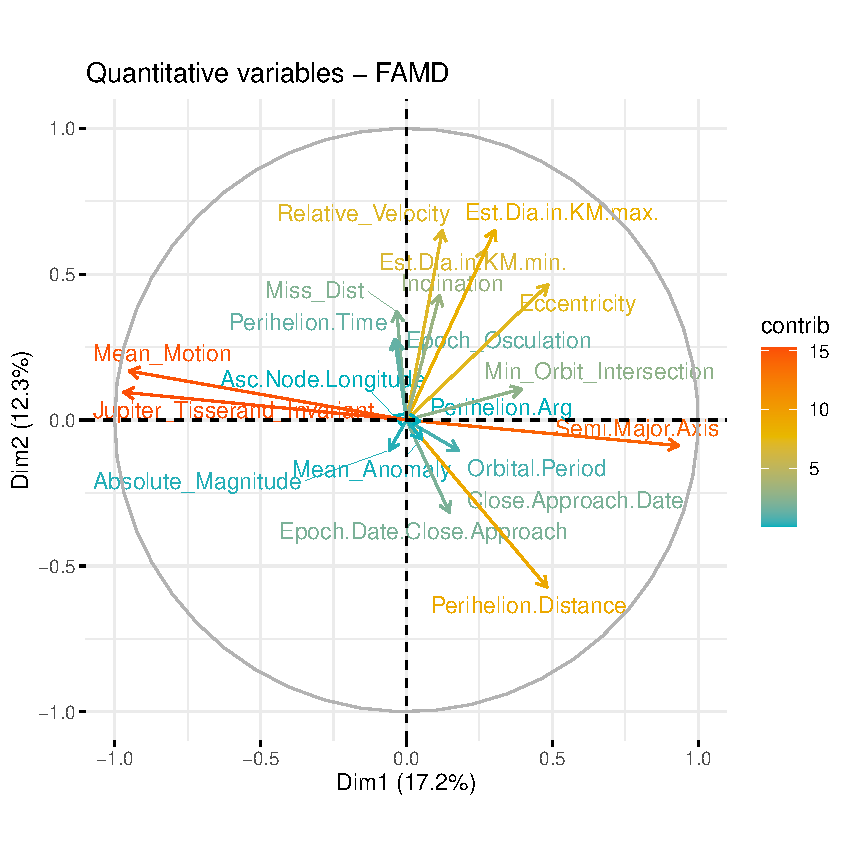
\includegraphics[width=1\textwidth]{Pic/FAMD_Quantitative variables.pdf}
\label{FAMD_Quantitative variables}
\end{center}
\end{figure}
\end{columns}
\end{frame}

\begin{frame}{Mutual information}
\begin{figure}
\begin{center}
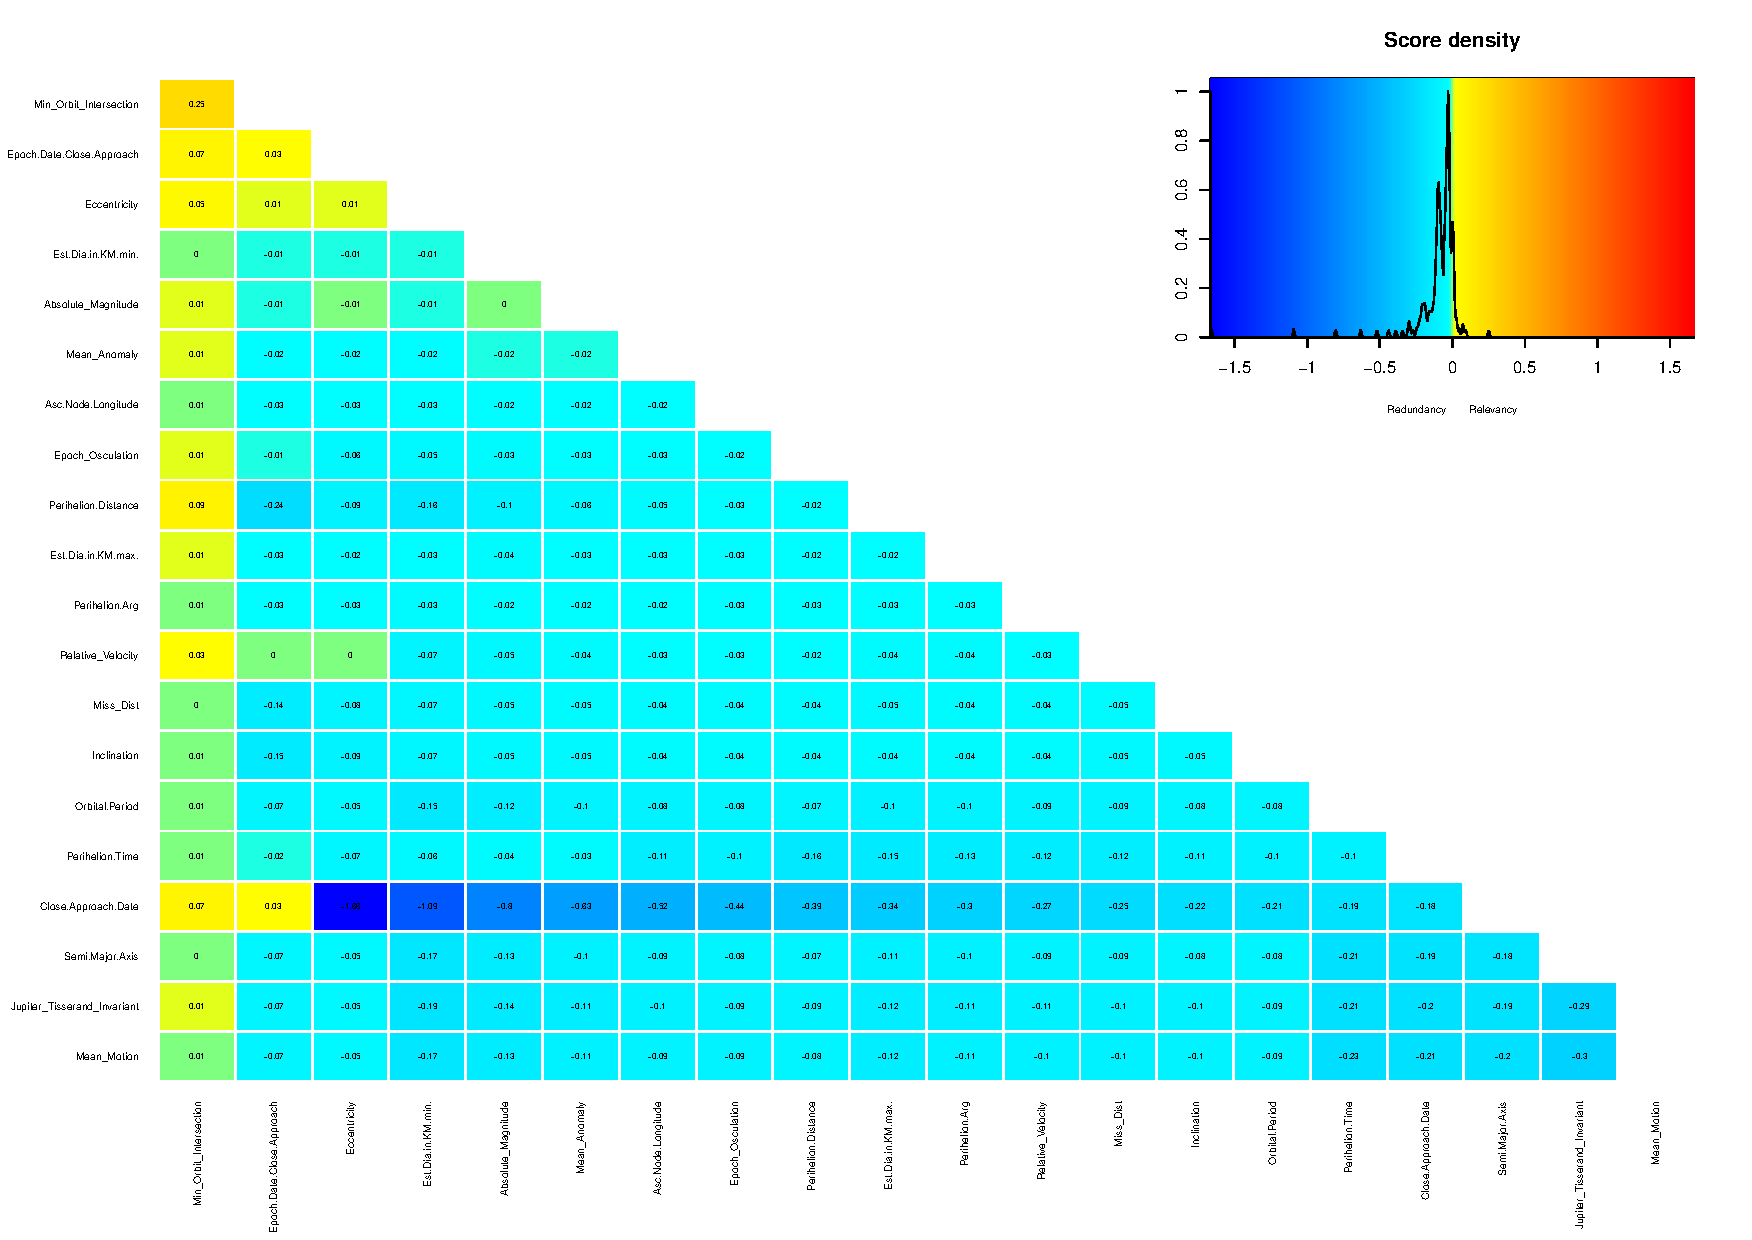
\includegraphics[width=0.9\textwidth]{Pic/Mutual_information.pdf}
\label{Mutual_information}
\end{center}
\end{figure}
\end{frame}

\section{Prob. models}

\begin{frame}{GLASSO}
\begin{columns}
\column{0.5\textwidth}
  \begin{figure}[b]{\textwidth}
    \centering
    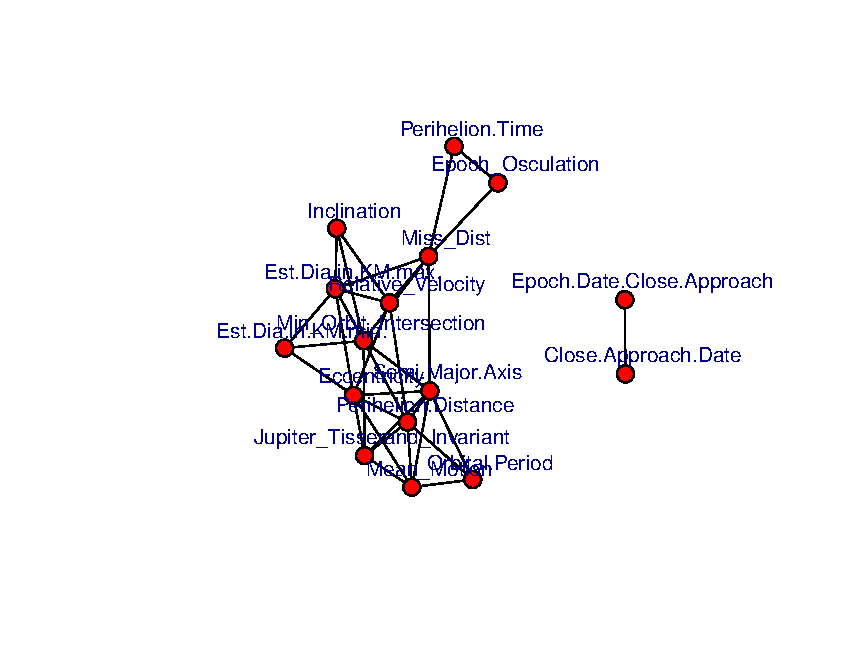
\includegraphics[width=\textwidth]{Pic/GLASSO_0.1.pdf}
    \subcaption{$\rho$=0.2 \begin{center}
    \end{center}}
  \end{figure} 
  \column{0.5\textwidth}
  \begin{figure}[b]{\textwidth}
    \centering
    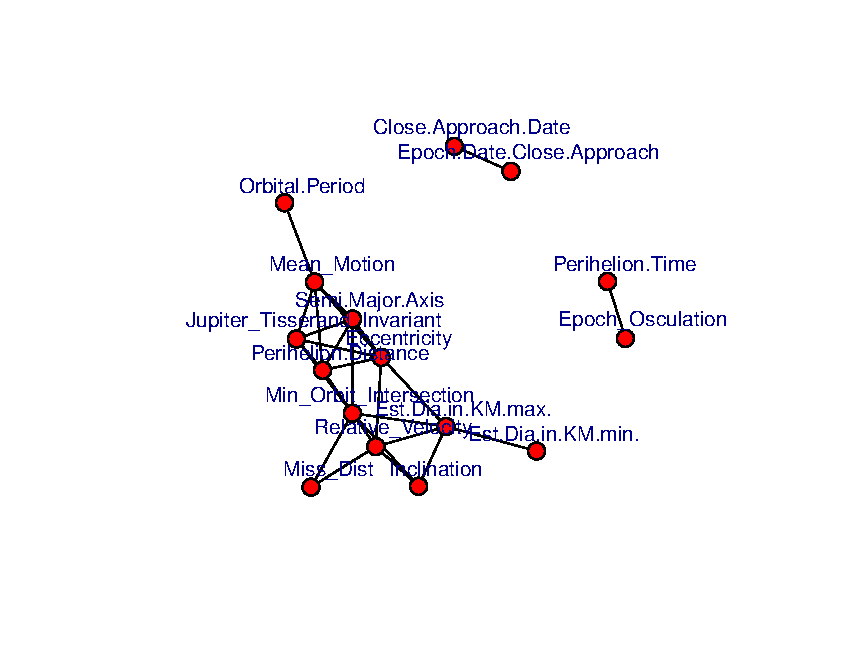
\includegraphics[width=\textwidth]{Pic/GLASSO_0.2.pdf}
    \subcaption{$\rho$=0.2 \begin{center}
    \end{center}}
  \end{figure}
\end{columns}
\end{frame}

\begin{frame}{GLASSO}
\begin{columns}
\column{0.5\textwidth}
  \begin{figure}[b]{\textwidth}
    \centering
    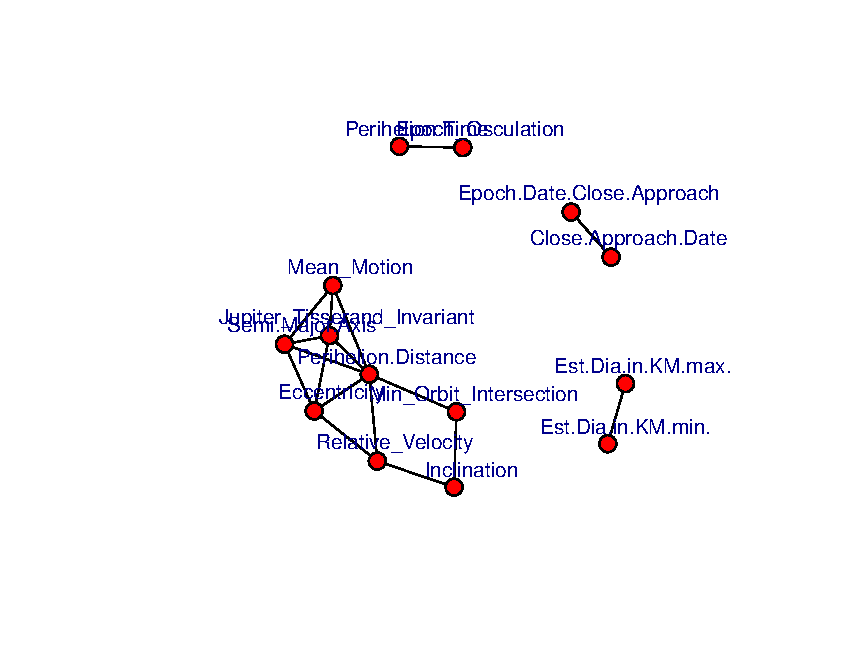
\includegraphics[width=\textwidth]{Pic/GLASSO_0.3.pdf}
    \subcaption{$\rho$=0.3 \begin{center}
    \end{center}}
  \end{figure} 
  \column{0.5\textwidth}
  \begin{figure}[b]{\textwidth}
    \centering
    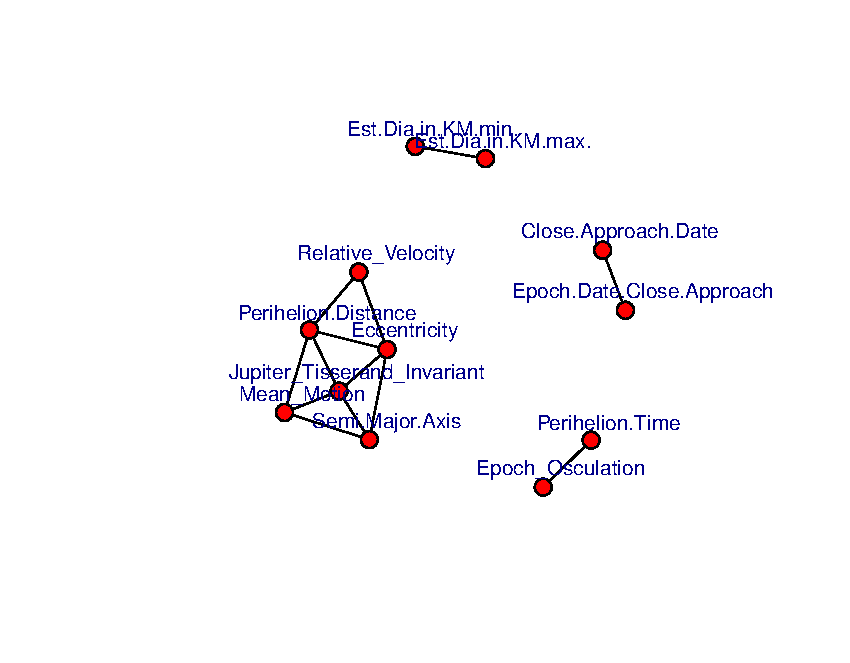
\includegraphics[width=\textwidth]{Pic/GLASSO_0.4.pdf}
    \subcaption{$\rho$=0.4 \begin{center}
    \end{center}}
  \end{figure}
\end{columns}
\end{frame}


\begin{frame}{Mixed interactions: mgm}
\begin{figure}[h]
\begin{center}
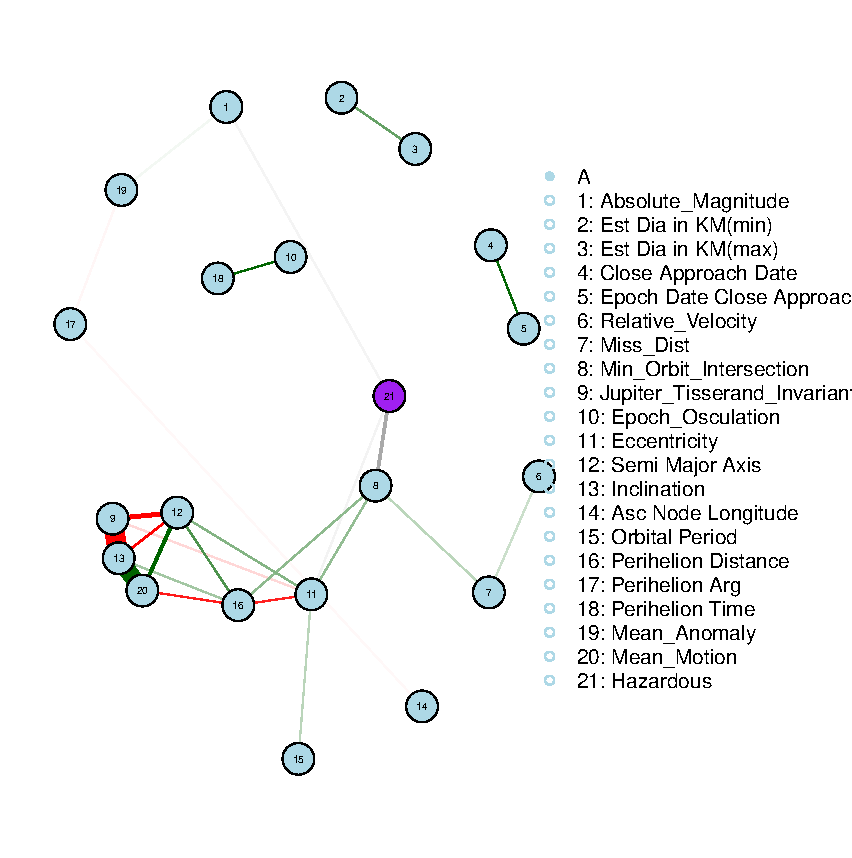
\includegraphics[width=0.6\textwidth]{Pic/mgm.pdf}
\label{mgm}
\end{center}
\end{figure}
\end{frame}

\begin{frame}{Mixed interactions: minforest}
\begin{figure}[h]
\begin{center}
\includegraphics[width=0.6\textwidth]{Pic/minforest.pdf}
\label{mgm}
\end{center}
\end{figure}
\end{frame}

\begin{frame}{Mixed interactions: mmod}
\begin{figure}[h]
\begin{center}
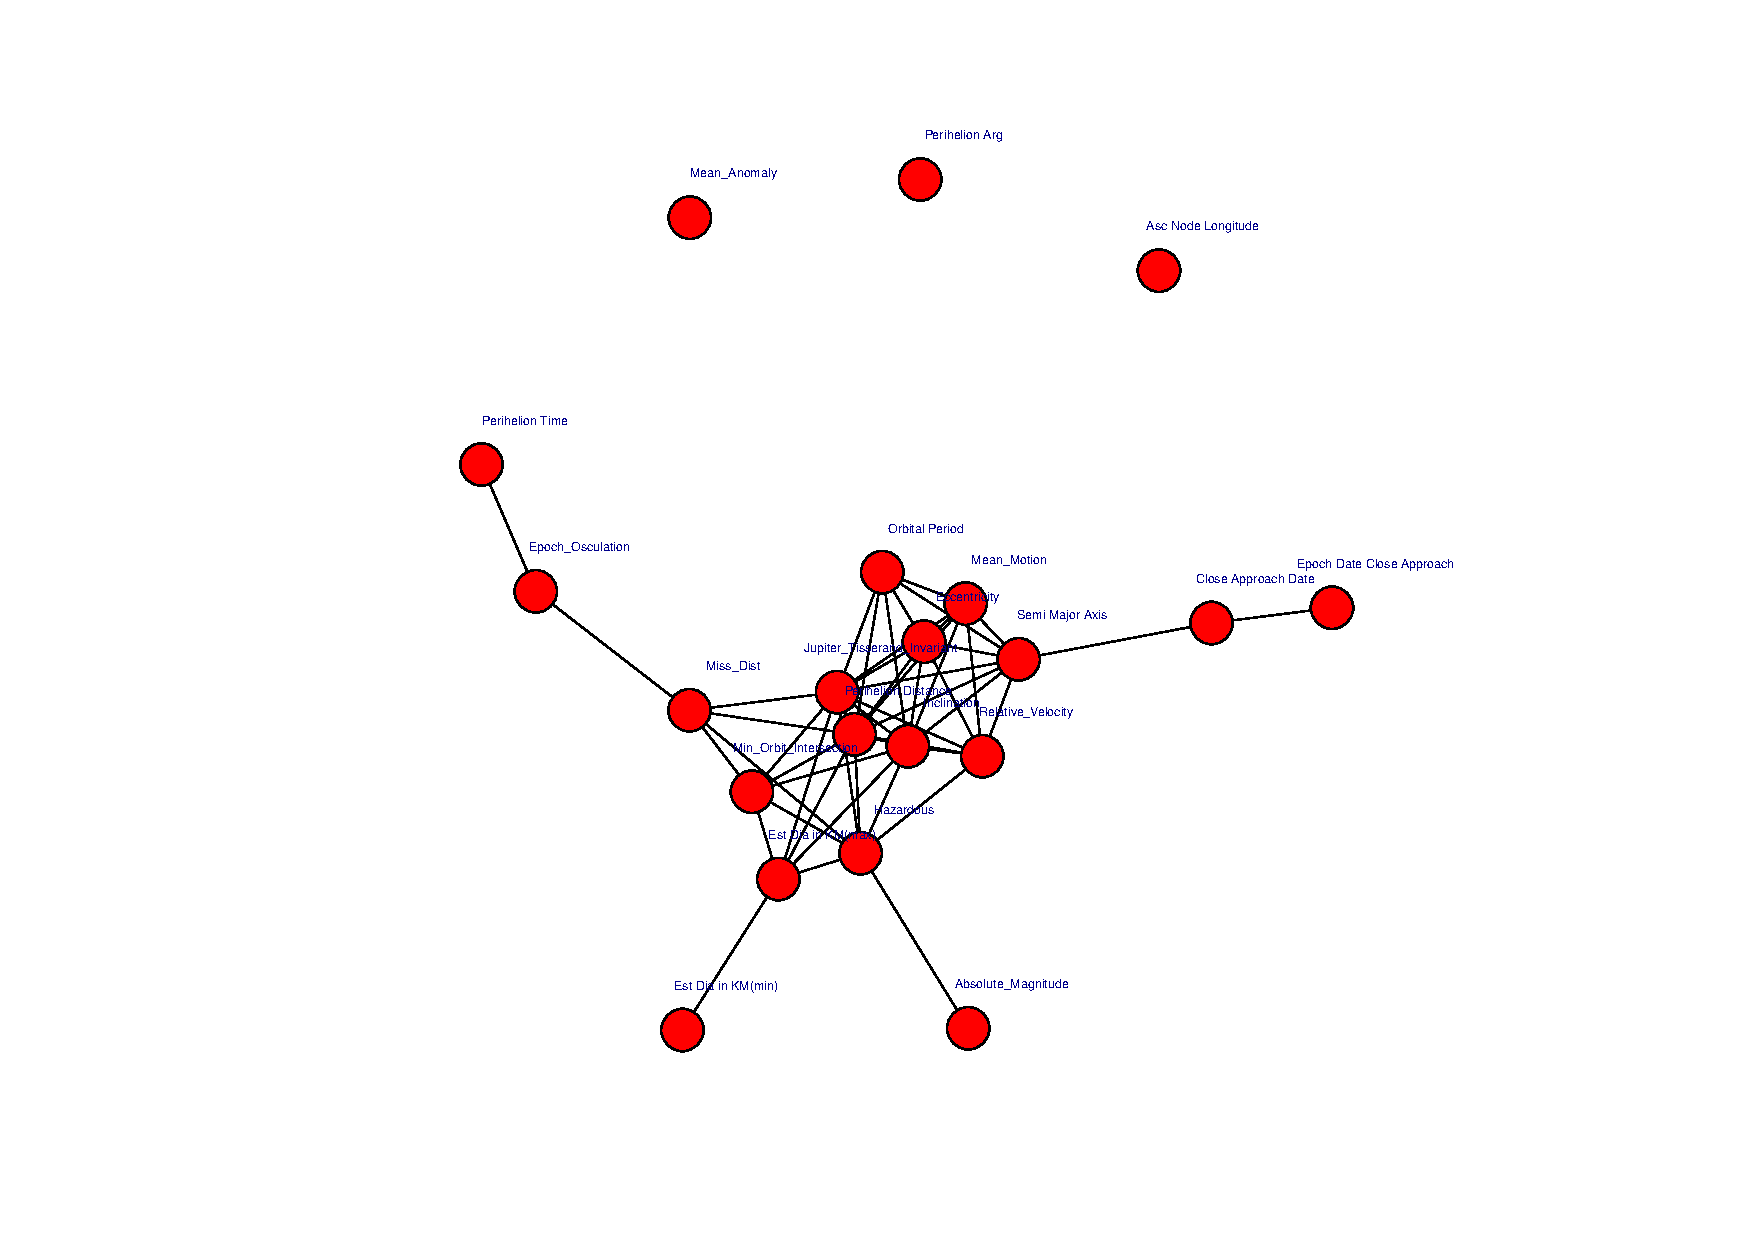
\includegraphics[width=0.6\textwidth]{Pic/mmod.pdf}
\label{mgm}
\end{center}
\end{figure}
\end{frame}

\begin{frame}{Mixed interactions}
The mgm model is the one that has the list of connection more coherent with the celestial mechanics laws. 
\begin{columns}
\column{0.5\textwidth}
  \begin{figure}[b]{\textwidth}
    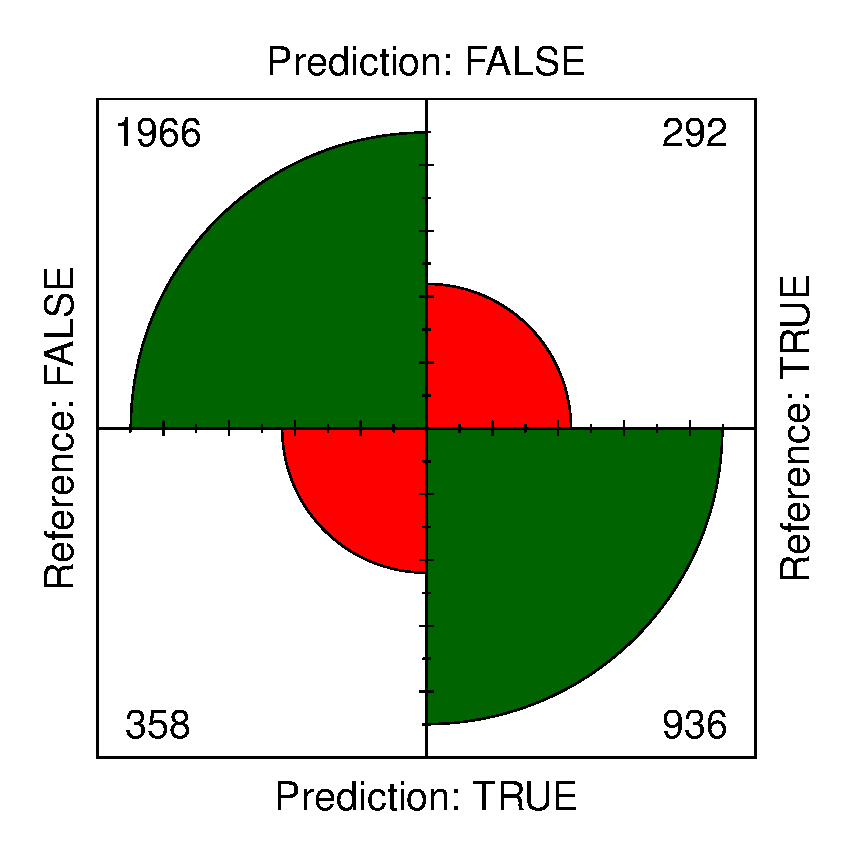
\includegraphics[width=\textwidth]{Pic/mgm_confusion.pdf}
  \end{figure} 
  \column{0.5\textwidth}
  \begin{figure}[b]{\textwidth}
    \includegraphics[width=\textwidth]{Pic/ROC_mgm.pdf}
  \end{figure}
\end{columns}
\end{frame}

\section{Other ML alg.}
\begin{frame}{Random Forest}
\begin{columns}
\column{0.5\textwidth}
  \begin{figure}[b]{\textwidth}
    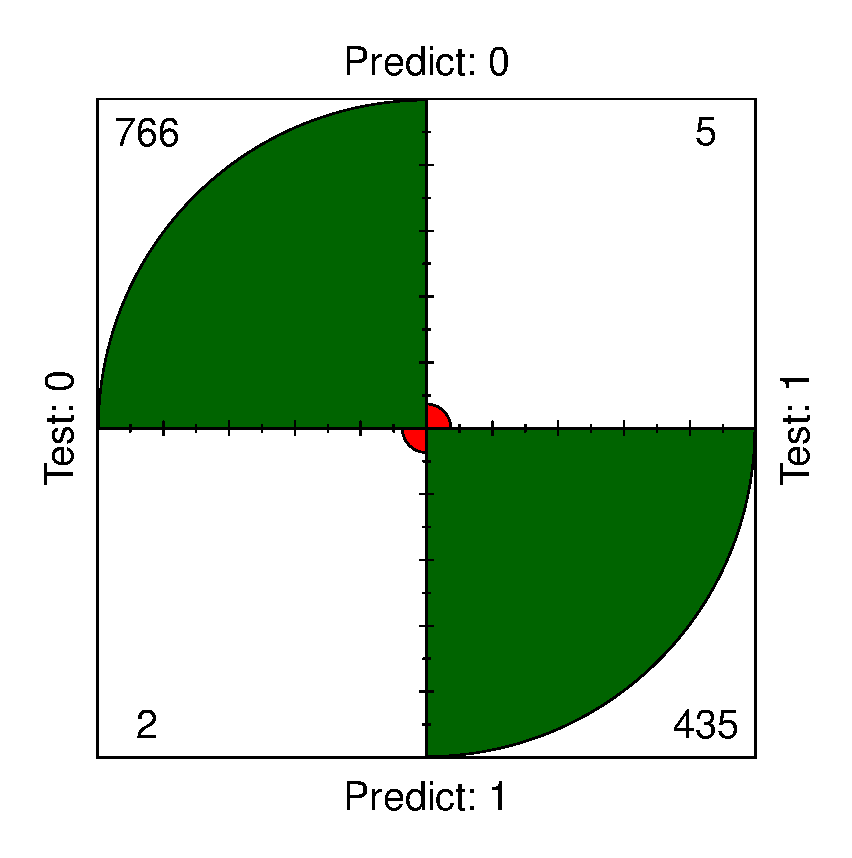
\includegraphics[width=\textwidth]{Pic/RF_confusion.pdf}
  \end{figure} 
  \column{0.5\textwidth}
  \begin{figure}[b]{\textwidth}
    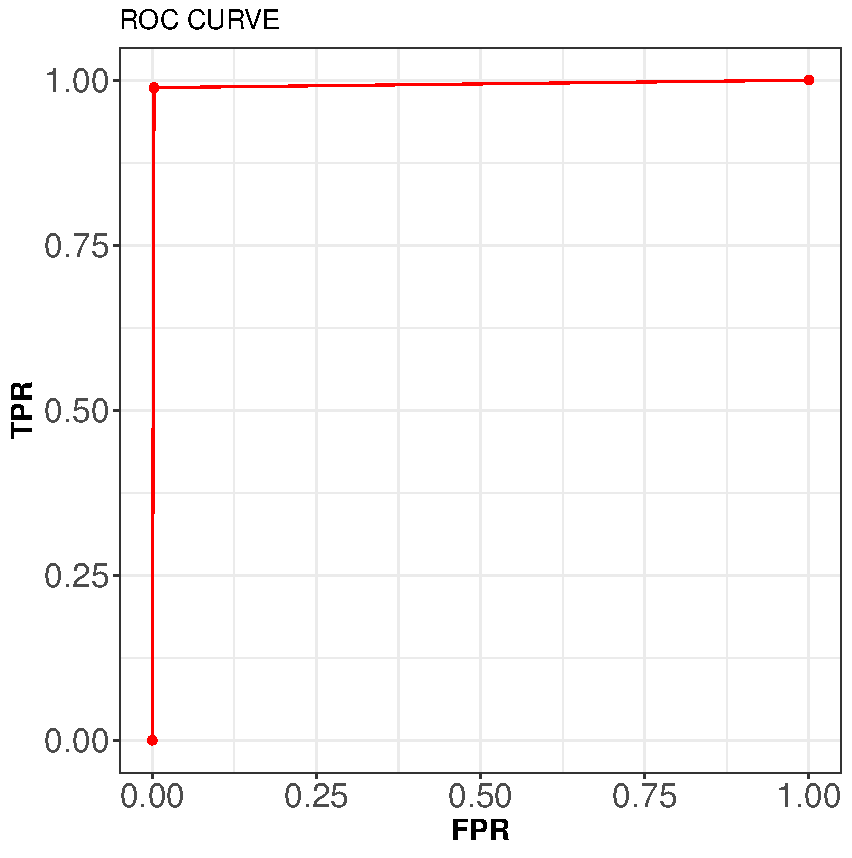
\includegraphics[width=\textwidth]{Pic/ROC_RF.pdf}
  \end{figure}
\end{columns}
\end{frame}

\begin{frame}{Random Forest}
  \begin{figure}[b]{\textwidth}
    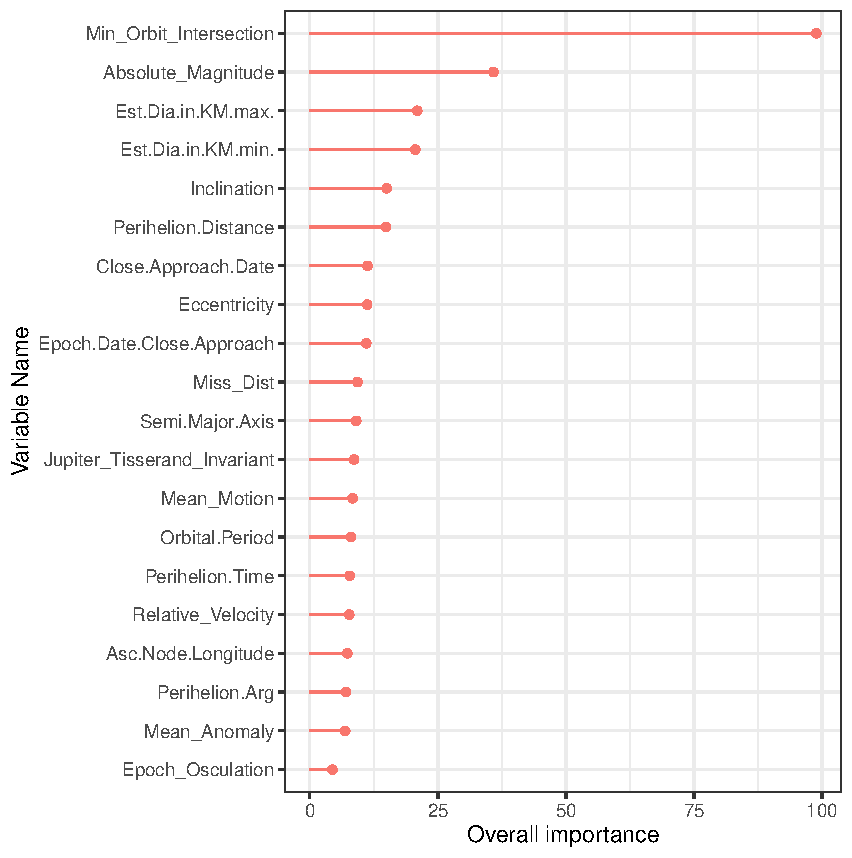
\includegraphics[width=0.7\textwidth]{Pic/RF_Importance.pdf}
  \end{figure} 
\end{frame}

\begin{frame}{Support Vector Machines}
\begin{columns}
\column{0.5\textwidth}
  \begin{figure}[b]{\textwidth}
    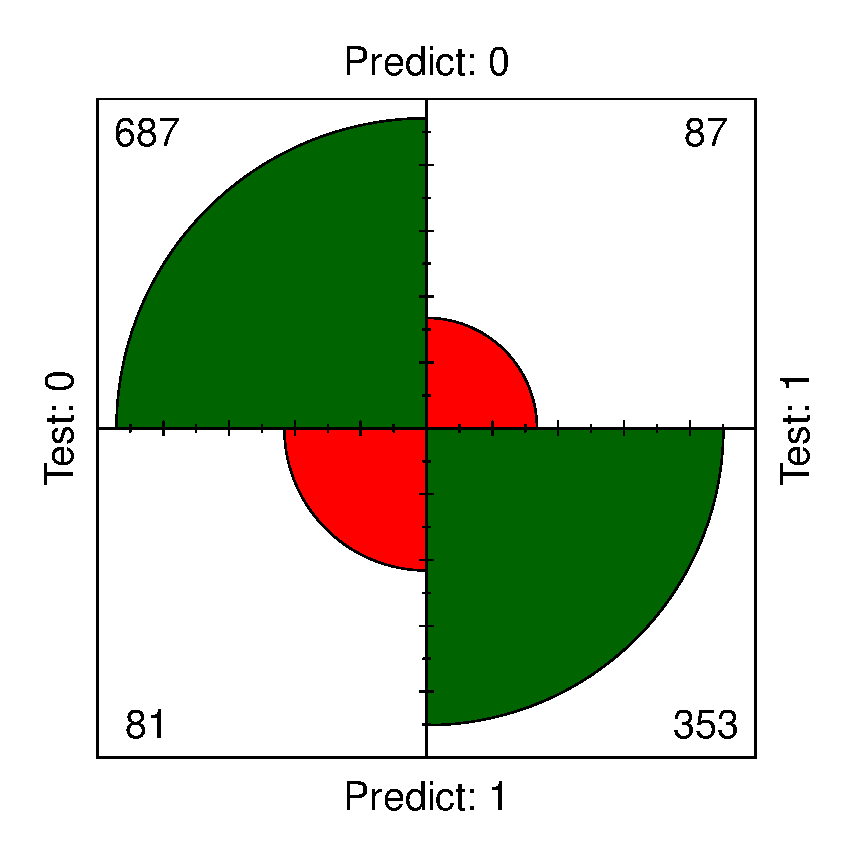
\includegraphics[width=\textwidth]{Pic/SVM_confusion.pdf}
  \end{figure} 
  \column{0.5\textwidth}
  \begin{figure}[b]{\textwidth}
    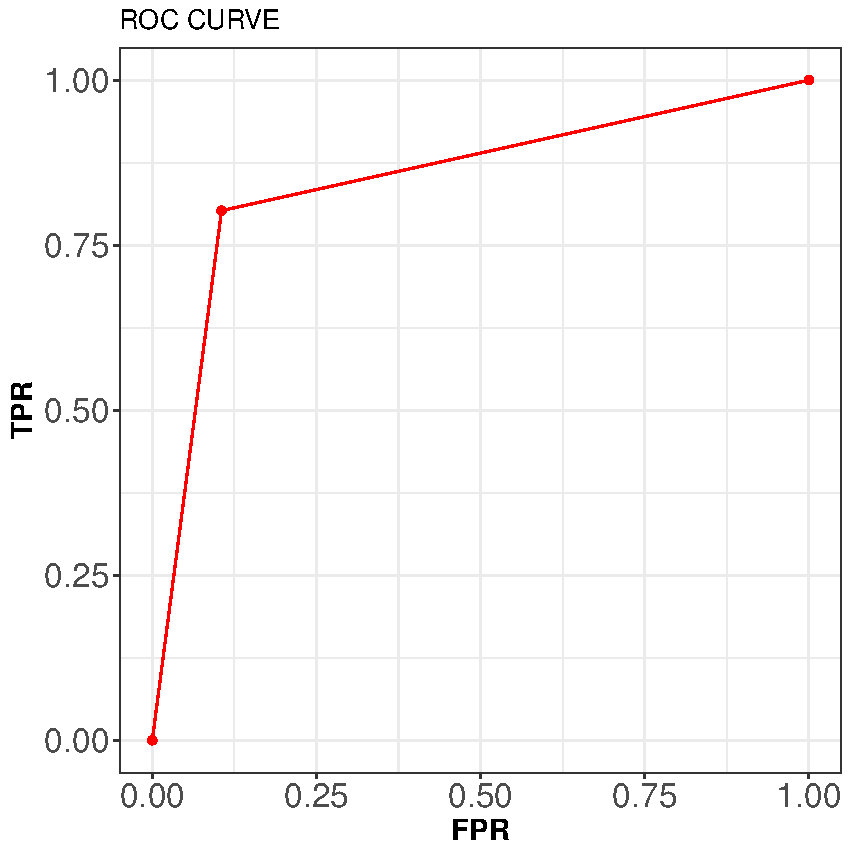
\includegraphics[width=\textwidth]{Pic/ROC_SVM.pdf}
  \end{figure}
\end{columns}
\end{frame}

\begin{frame}{Quadratic Discriminant Analysis (QDA)}
\begin{columns}
\column{0.5\textwidth}
  \begin{figure}[b]{\textwidth}
    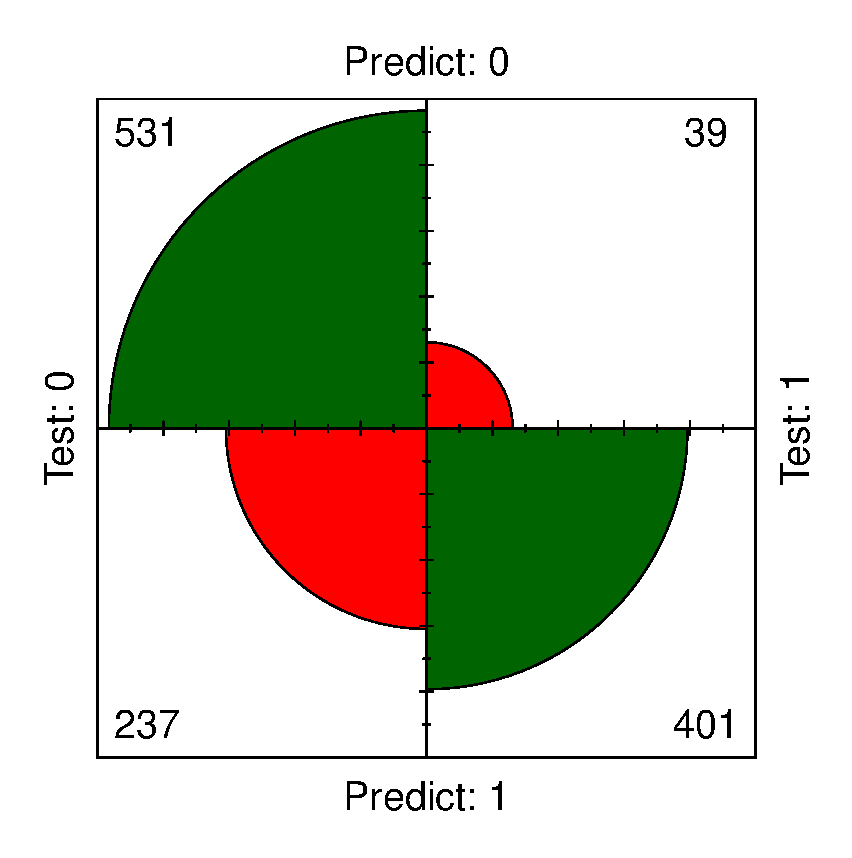
\includegraphics[width=\textwidth]{Pic/QDA_confusion.pdf}
  \end{figure} 
  \column{0.5\textwidth}
  \begin{figure}[b]{\textwidth}
    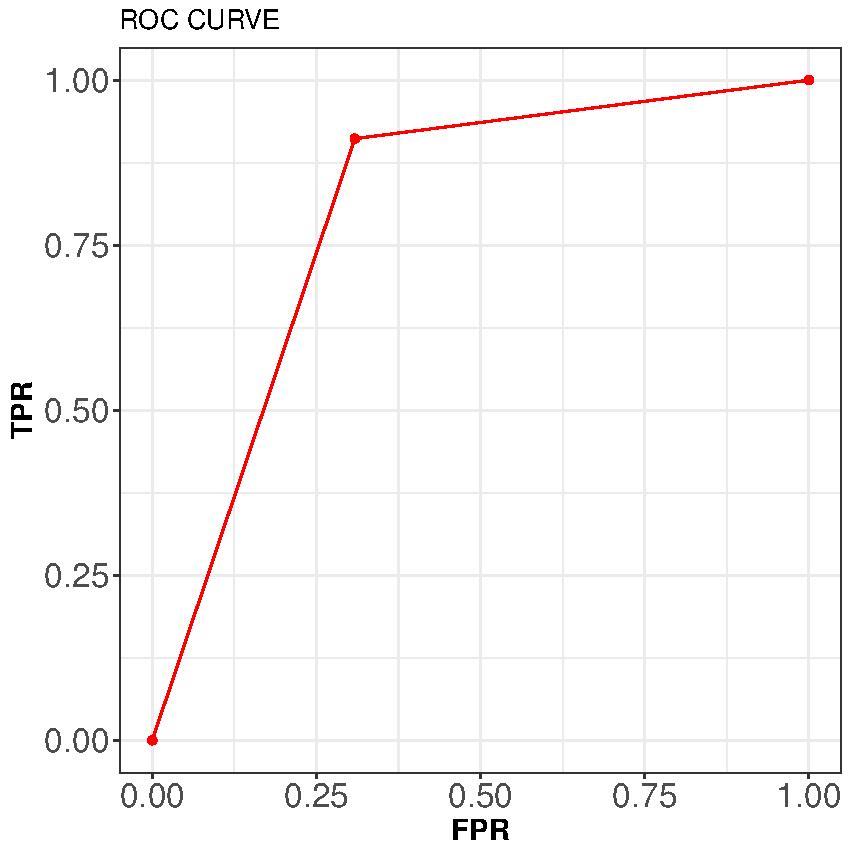
\includegraphics[width=\textwidth]{Pic/ROC_QDA.pdf}
  \end{figure}
\end{columns}
\end{frame}

\begin{frame}{Logistic regression}
\begin{columns}
\column{0.5\textwidth}
  \begin{figure}[b]{\textwidth}
    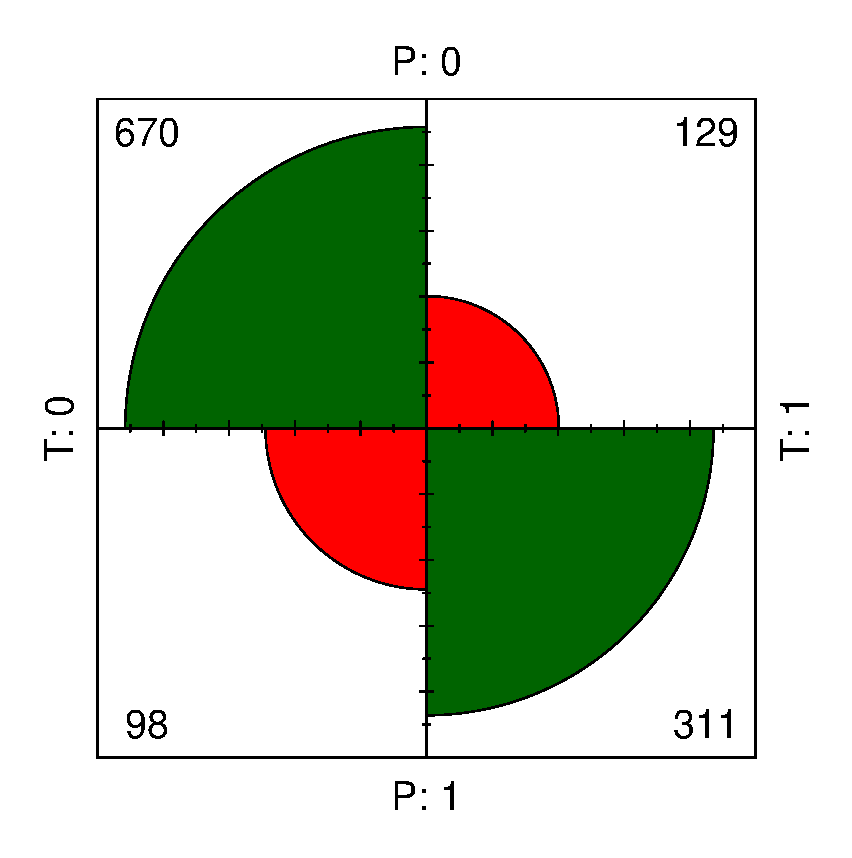
\includegraphics[width=\textwidth]{Pic/Logisic_confusion.pdf}
  \end{figure} 
  \column{0.5\textwidth}
  \begin{figure}[b]{\textwidth}
    \includegraphics[width=\textwidth]{Pic/ROC_Logistic.pdf}
  \end{figure}
\end{columns}
\end{frame}


\begin{frame}{$\phi$ coefficient}
\begin{table}[]
\caption{$\phi$ coefficient (also known as Matthews correlation coefficient )}
\begin{center}
\begin{tabular}{c|c}
Algorithm & $\phi$ \\ \hline
RF        & 0.9876 \\ \hline
SVM       & 0.7111 \\ \hline
logistic  & 0.6173 \\ \hline
mgm       & 0.5997 \\ \hline
QDA       & 0.5562 
\end{tabular}
\end{center}
\label{phi_values}
\end{table}
\end{frame}

\section{Conclusions}

\begin{frame}{Conclusions: forecast performances vs intepretability}
\begin{itemize}
\item The mgm algorithm is not the best one in term of performances, but it provides the connections between the features. On the other side, except for the variable importance in RF, the other are black box one
\item The mgm model, as the other graphical model is open to a true scientific validation, the other not. 
\item The probabilistic models lack in the forecast is definitely compensated by their interetability 
\item This is meaningful since this two features are in conflict 
\item The probabilistic models provide a good trade-off between intepretability and forecast performances, as long as one is interest to produce a really scientific result (e.g if the only aim is the forecast the RF is definitely better. However how long one can trust to the RF result ?)
\end{itemize}
\end{frame}

\section{SI}

\begin{frame}{Introduction}

\end{frame}

\begin{frame}{Introduction}

\end{frame}

\begin{frame}{Introduction}

\end{frame}
\begin{frame}{Introduction}

\end{frame}
\begin{frame}{Introduction}

\end{frame}
\begin{frame}{Introduction}

\end{frame}

\begin{frame}{Introduction}

\end{frame}
\begin{frame}{Introduction}

\end{frame}
\begin{frame}{Introduction}

\end{frame}
\begin{frame}{Introduction}

\end{frame}
\begin{frame}{Introduction}

\end{frame}
\begin{frame}{Introduction}

\end{frame}
\begin{frame}{Introduction}

\end{frame}
\begin{frame}{Introduction}

\end{frame}

\begin{frame}{Ref}
\printbibliography
\end{frame}



\end{document}